\section{Задание 2. Графическое решение ДУ первого порядка}

\textbf{Условие.}

В задачах проведите исследование:
\begin{enumerate}
    \item Изучите по источникам метод изоклин (например, здесь: Романко, В. К. Курс дифференциальных уравнений и вариационного исчисления — URL:https://e.lanbook.com/book/152035).

    \item Постройте приближенно семейство интегральных кривых данного ДУ методом изоклин.

    \item Решите задачу аналитически. Изобразите точное решение.

    \item Сравните точное и приближенное решение.
\end{enumerate}

\[y^\prime = \frac{y}{x + y}\]

\vspace{10mm}
\textbf{Решение.}

\begin{enumerate}
    \item Метод изоклин состоит в следующем:

    \begin{itemize}
        \item Строится достаточно густая сетка изоклин для различных значений k и на каждой изоклине изображаются небольшие отрезки с наклоном k.

        \item Начиная из точки (x\textsubscript{0}, y\textsubscript{0}), поводится линия, которая, будет пересекать каждую изоклину под углом, заданным полем направлений.
        Полученная таким образом кривая и будет приближенным изображением интегральной кривой уравнения, проходящей через точку (x\textsubscript{0}, y\textsubscript{0}).
    \end{itemize}

    \item Изоклины, которые задает это уравнение, описываются уравнением $\frac{y}{y + x} = k \Longleftrightarrow y = \frac{kx}{k - 1}$ - множество прямых, пересекающихся в начале координат

    Прямые в 1 и 3 четвертях задают наклон кривой $k \in (0; 1)$, во 2 и 4 четвертях - наклон $k \in (-\infty; 0) \union (1; \infty)$.

    Используя компьютерные технологии (язык программирования Python и библиотека для изображения графиков matplotlib),
    построим несколько изоклин и 3 интегральные кривые, которые они задают:

    \begin{center}
        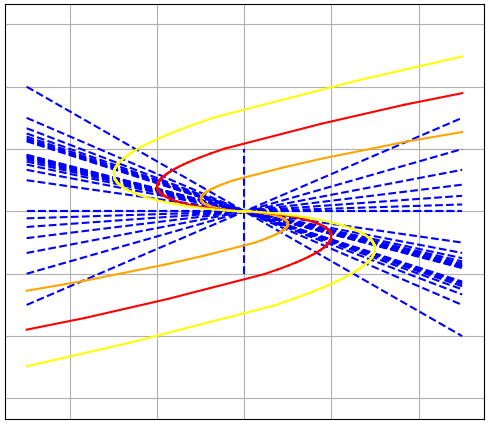
\includegraphics[height=80mm]{images/2a1}
    \end{center}

    \item Решим дифференциальное уравнение:

    $\displaystyle
    y^\prime = \frac{y}{x + y}\\
    \frac{dy}{dx} = \frac{y}{x} \cdot \frac{1}{1 + \frac{y}{x}}\\
    \frac{dy}{dx} = t \cdot \frac{1}{1 + t}\\
    t^\prime x + t = t \cdot \frac{1}{1 + t}\\
    t^\prime x = \frac{-t^2}{1 + t}\\
    \frac{(1 + t)dt}{-t^2} = \frac{dx}{x}\\
    \frac{dt}{-t^2} + \frac{tdt}{-t^2} = \frac{dx}{x}\\
    d\frac{1}{t} + \left(-\frac{1}{2}d \ln |t^2|\right) = d\ln |x|\\
    \frac{1}{t} + (-\ln |t|) = \ln |x| + C\\
    \frac{x}{y} - \ln |\frac{y}{x}| = \ln |x| + C\\
    \frac{x}{y} - \ln |y| = C\\
    $


    \item Построим в Geogebra уравение выше с 3 разными константами:

    \begin{center}
        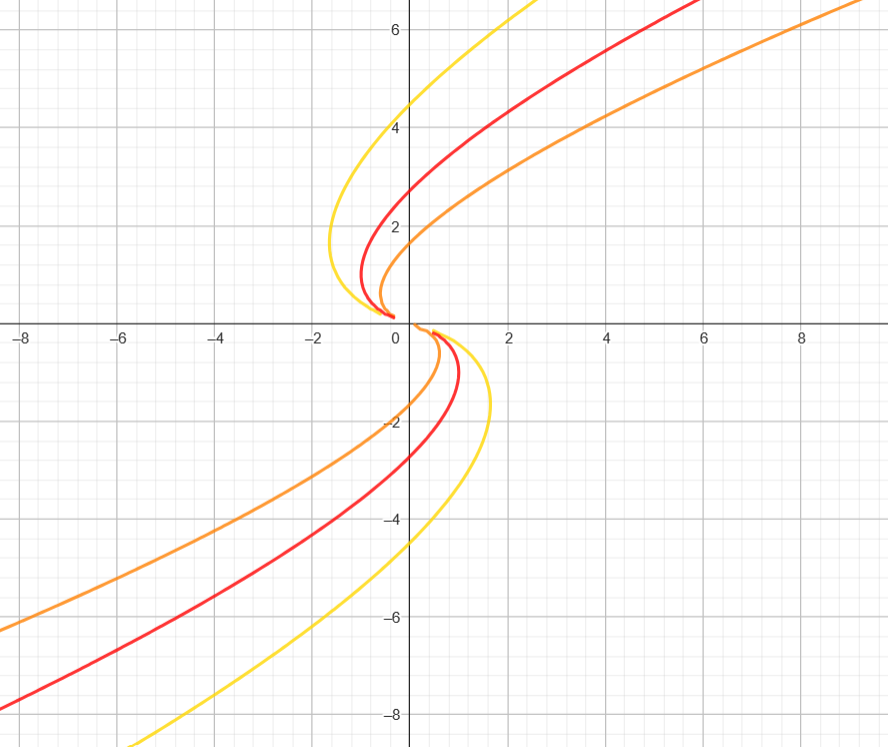
\includegraphics[height=80mm]{images/2a2}
    \end{center}

    Как можем заметить, метод изоклин дает довольно точное изображение того, как ведет себя семейство интегральных кривых
\end{enumerate}

